\documentclass[../mathNotesPreamble]{subfiles}

\providecommand{\relscalefact}{1.4}
\begin{document}
\relscale{\relscalefact}
  \section{1.1: Functions and Function Notation}

  \begin{defn*}
    A \textbf{function} is a relation in which each possible input value leads to exactly one output value.

    The input values make up the \textbf{domain}, and the output values make up the \textbf{range}.
  \end{defn*}

  \noindent
  \begin{minipage}{0.495\linewidth}
    \newcommand{\funcMachine}{--++(0,-vert) --++(dx,-dy) |- ++(-a,-vert) |- ++(c,-h)
      -- ++(0,-vert) --++(-dx, -dy) {[sharp corners] --++(0,-vert-vgap) %bottom left portion
      --++(b+2*dx,0)} --++(0,vert+vgap) --++(-dx,dy) |- ++(a,vert)
      -- ++(0,h) -| ++(-c,vert) --++(dx,dy) --++(0,vert); %top right portion
    }
    \centering
    %bottom left corner is (0,0)
    %a,b,c are widths representing left wall to chute, width of chute, chute to right wall
    %h is height of rectangle
    %dx, dy control slope of "funnel"
    %vert is the height of straight parts of "funnel"
    %paths start at top left (on "funnel")
    \begin{tikzpicture}[declare function={
      a=1.25; b=1.25; c=5.5;
      dx=0.9*a; dy=0.6*a;
      h=1.75; vert=0.6; vgap=0.2;}]
      \tikzalt{Diagram of a function machine}
      \begin{scope}
        \clip (-0.1+0,h+2*vert+dy) rectangle ++(0.2+a+b+c,-4*vert-2*dy-h);
        \draw[line width=1pt, fill=lander_blue!25, rounded corners=6pt]
          (a-dx,h+2*vert+dy) \funcMachine
      \end{scope}
      \node (Input) [align=center] at ({a+b/2},{h+vert+dy}) {Input\\$x$};
      \node[align=center] at ({(a+b+c)/2},{h/2}) {$f$};
      \node (Output) [align=center] at ({c+b/2},{-vert-dy}) {$f(x)$\\Output};

      \draw[->] (Input) -- ++(0,-vert-dy);
      \draw[<-] (Output) -- ++(0,vert+dy);
    \end{tikzpicture}
  \end{minipage}\hfill%
  \begin{minipage}{0.495\linewidth}
    \begin{center}
      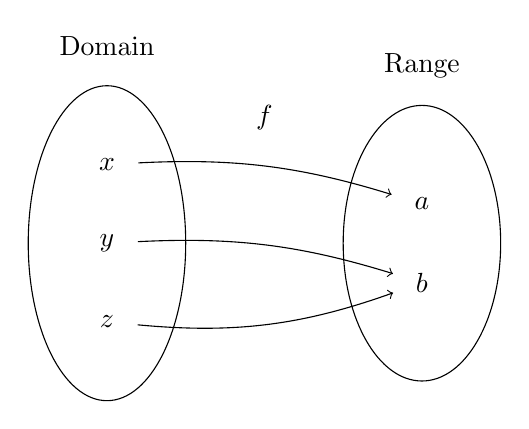
\begin{tikzpicture}
        \tikzalt{Ellipses demonstrating a function mapping from domain to range}
        \draw (-2,0) circle [x radius=1, y radius=2];
        \node at (-2,2.5) {Domain};
        \draw (2,0) circle [x radius=1, y radius=1.75];
        \node at (2,2.25) {Range};
        \node (xo) at  (-2,1)   {$x$};
        \node (xt) at  (-2,0)   {$y$};
        \node (xr) at  (-2,-1)  {$z$};
        \node (fxo) at (2,0.5)  {$a$};
        \node (fxt) at (2,-0.5) {$b$};
        \node at (0,1.6) {$f$};
        \draw[->, shorten >=5pt, shorten <=5pt] (xo) to [bend left=10] (fxo);
        \draw[->, shorten >=5pt, shorten <=5pt] (xt) to [bend left=10] (fxt);
        \draw[->, shorten >=5pt, shorten <=5pt] (xr) to [bend right=12.5] (fxt);
      \end{tikzpicture}
    \end{center}
  \end{minipage}

  \begin{ex*}
    Let $f(x)=2x^2-2x+1$. Evaluate the following
  \end{ex*}
  \begin{extasks}[after-item-skip=\stretch{1}](3)
    \task $f(1)$
    \task $f(-2)$
    \task $f(a)$
    \task $f(a+h)$
    \task* $\dfrac{f(a+h)-f(a)}{h}$
  \end{extasks}
  \vspace*{\stretch{1}}
  \pagebreak

  \begin{ex*}
    Suppose that the following tables represent a carnival truck's menu prices. Which table would represent a valid function?
  \end{ex*}

  \hspace*{\stretch{0.25}}
  \begin{tabular}{@{}lr@{}}\toprule
    Item& Price\\ \midrule
    Funnel cake& \$8\\
    Chicken strips& \$9\\
    Ribbon fries& \$7\\
    Cheese nachos& \$6\\
    \bottomrule
  \end{tabular}\hspace*{\stretch{1}}
  \begin{tabular}{@{}lr@{}}\toprule
    Item& Price\\ \midrule
    Funnel cake& \$8\\
    Chicken strips& \$8\\
    Ribbon fries& \$7\\
    Cheese nachos& \$6\\
    \bottomrule
  \end{tabular}\hspace*{\stretch{1}}
  \begin{tabular}{@{}lr@{}}
    \toprule
    Item& Price\\ \midrule
    Funnel cake& \$8\\
    Chicken strips& \$8\\
    Ribbon fries& \$8\\
    Funnel cake& \$6\\
    \bottomrule
  \end{tabular}
  \hspace*{\stretch{0.25}}
  \vspace*{\stretch{0.5}}

  \begin{ex*}
    Based on an old match-makers rule, the socially ``acceptable'' minimum age of someone you can date is half your age plus seven. Make a function that takes your age, $x$, and finds the minimum age of someone you can date, $y$.
  \end{ex*}
  \vspace*{\stretch{0.5}}
  \pagebreak

  \begin{ex*}
    Create a table to represent a function that takes each month and returns the number of days (in a non-leap year).
  \end{ex*}
  \vspace*{\stretch{1}}

  \begin{ex*}
    If possible, express the relationship $2n+6p=12$ as a function $p=f(n)$. Graph the result.
  \end{ex*}
  \vspace*{\stretch{1}}

  \begin{ex*}
    If possible, express the relationship $x^2+y^2=1$ as a function $y=f(x)$. Graph the result.
  \end{ex*}
  \vspace*{\stretch{1}}
  \pagebreak

  \begin{defn*}[Vertical Line Test]
    A curve in the $xy$-plane is the graph of a function $y=f(x)$ (an explicit function) if and only if each vertical line intersects it in at most one point
  \end{defn*}

  \begin{ex*}
    Use the vertical line test on the following graphs to determine which graphs may represent an explicit function:
  \end{ex*}

  \begin{center}
    \begin{tabular}{c@{\hspace*{40pt}}c}
      \begin{tikzpicture}[declare function={
        f(\x)=(\x-1.5)*(\x+1)*(\x+2)+6;}]
        \tikzalt{A graph of a cubic function}
        \begin{axis}[
          axis lines=center,
          axis line style={black,->},
          xmajorticks=false,
          ymajorticks=false,
          xmin=-3.25, xmax=3.25,
          enlargelimits={value=0.025, auto},
          ticklabel style={font=\footnotesize,inner sep=0.5pt,fill=white,opacity=1.0, text opacity=1},
          xlabel=$x$, xlabel style={at={(ticklabel* cs:1)},anchor=north west},
          ylabel=$y$, ylabel style={at={(ticklabel* cs:1)},anchor=south west},
          every axis plot/.append style={domain=xmin:xmax, line width=0.95pt, color=lander_blue, samples=255},
          ]
          \addplot[<->] expression[domain=-3:2.25]{f(x)};
        \end{axis}
      \end{tikzpicture} &
      \begin{tikzpicture}
        \tikzalt{A graph of a non-explicit function}
        \begin{axis}[
          axis lines=center,
          axis line style={black,->},
          xmajorticks=false,
          ymajorticks=false,
          xmin=-4, xmax=4,
          ymin=-1, ymax=5,
          enlargelimits={value=0.025, auto},
          ticklabel style={font=\footnotesize,inner sep=0.5pt,fill=white,opacity=1.0, text opacity=1},
          xlabel=$x$, xlabel style={at={(ticklabel* cs:1)},anchor=north west},
          ylabel=$y$, ylabel style={at={(ticklabel* cs:1)},anchor=south west},
          every axis plot/.append style={domain=xmin:xmax, line width=0.95pt, color=lander_blue, samples=255},
          ]
          \draw[samples=255, line width=0.95pt, lander_blue, domain=0.2:3.8, <->] plot({(\x-1)*(\x-2)*(\x-3)},{\x});
        \end{axis}
      \end{tikzpicture}\\[2\baselineskip]
      \begin{tikzpicture}[declare function={
        f(\x)=sqrt(\x^2-1);}]
        \tikzalt{A graph of a discontinuous function}
        \begin{axis}[
          axis lines=center,
          axis line style={black,->},
          xmajorticks=false,
          ymajorticks=false,
          ymax=10,
          enlargelimits={value=0.025, auto},
          ticklabel style={font=\footnotesize,inner sep=0.5pt,fill=white,opacity=1.0, text opacity=1},
          xlabel=$x$, xlabel style={at={(ticklabel* cs:1)},anchor=north west},
          ylabel=$y$, ylabel style={at={(ticklabel* cs:1)},anchor=south west},
          every axis plot/.append style={domain=xmin:xmax, line width=0.95pt, color=lander_blue, samples=255},
          ]
          \addplot[<-] expression[domain=-5:-1]{f(x)};
          \addplot[->] expression[domain=1:5]{f(x)};
        \end{axis}
      \end{tikzpicture}&
      \begin{tikzpicture}[declare function={
        g(\x)=1.25*(abs(\x)-1);
        f(\x)=g(\x)<=0 ? sqrt(1-x^2) : g(\x);}]
        \tikzalt{A graph of a continuous, non-differentiable function}
        \begin{axis}[
          axis lines=center,
          axis equal,
          axis line style={black,->},
          xmajorticks=false,
          ymajorticks=false,
          enlargelimits={value=0.025, auto},
          ticklabel style={font=\footnotesize,inner sep=0.5pt,fill=white,opacity=1.0, text opacity=1},
          xlabel=$x$, xlabel style={at={(ticklabel* cs:1)},anchor=north west},
          ylabel=$y$, ylabel style={at={(ticklabel* cs:1)},anchor=south west},
          every axis plot/.append style={domain=xmin:xmax, line width=0.95pt, color=lander_blue, samples=255},
          ]
          \addplot[<->] expression[domain=-2:2, samples=511]{f(x)};
        \end{axis}
      \end{tikzpicture}
    \end{tabular}
  \end{center}

  \pagebreak

  \begin{defn*}[One-to-One]
    The \textbf{horizontal line test} determines if every horizontal line passes through the graph of a function in at most one point.

    A function is said to be \textbf{one-to-one} if each output value corresponds to \emph{exactly} one input value (and hence passes the horizontal line test).
  \end{defn*}
  \begin{ex*}
    Which of the following represent a one-to-one function?
    \hspace*{\stretch{1}} %DESMOS math 114: one-to-one functions
    \href{https://www.desmos.com/calculator/s2h0fl2ahx}{\textcolor{blue}{\underline{Graph}}}
  \end{ex*}
  \begin{extasks}[after-item-skip=\stretch{1}](2)
    \task $y=x^2 $
    \task $y^2=x$
    \task $f(x)=\sqrt{x}$
    \task $y=\abs{x}$
    \task $f(x)=(x+1)(x-1)(x-2)$
    \task The equation of a circle:\\ $x^2+y^2=1$
    \task The area of a circle:\\ $A=\pi r^2$
  \end{extasks}
  \vspace*{\stretch{1}}
  \vspace*{-\baselineskip}
  \hspace*{\stretch{1}}\href{https://openstax.org/books/precalculus-2e/pages/1-1-functions-and-function-notation#Table_01_01_14}{\textcolor{blue}{\underline{Graphs of basic functions}}}

  \pagebreak
\end{document}
